\section{Измерение параметров устройств.}

Одним из основных параметров, влияющих на конкурентоспособность системы, является дальность связи, которую можно увеличить за счёт увеличения выходной мощности и улучшения чувствительности приемного тракта. В то же время для получения разрешения на работу изделия должны удовлетворять ограничениям на полосу частот и выходную мощность, устанавливаемым действующим законодательством. Для контроля этих параметров были разработаны следующие методики измерений.

\subsection{Средства измерений, вспомогательное оборудование и программное обеспечение.}

Для измерения параметров передаваемого сигнала потребуется анализатор спектра либо векторный анализатор цепей (ВАЦ).
Для измерения параметров приемного тракта потребуется генератор сигнала произвольной формы и анализатор спектра либо ВАЦ. 
В данной методике будет описан процесс измерения с использованием анализатора спектра Rohde\&Schwarz FSEB и генератора сигнала Rohde\&Schwarz SMU200A. 
Для автоматизации измерений все исследуемые устройства будут подключены к ПК с установленным ПО для управления СИ и терминалом последовательного порта для управления ИУ. Также потребуется специальное ПО с поддержкой AT-команд для исследуемых устройств.

\subsection{Измерение параметров выходного тракта.}

\begin{figure}[H]
	\centering
	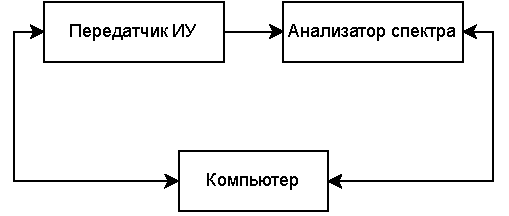
\includegraphics[width=0.7\textwidth,keepaspectratio]{TransmitterMeasSch.pdf}
	\caption{Схема установки измерения параметров передаваемого сигнала.}
	\label{fig:TransmitterMeasSch}
\end{figure}

\subsubsection{Подготовка к проведению измерений}

\begin{enumerate}
	\setlength\itemsep{-1ex}
	\item Включить ПК 
	\item Включить анализатор спектра. Прогреть в течение 15 минут.
	\item Откалибровать анализатор спектра
	\begin{enumerate}
		\item Открыть меню калибровки нажав кнопку CAL в разделе SYSTEM
		\item Запустить процесс калибровки, выбрав пункт SHORT CAL.
		\item Дождаться окончания процесса калибровки
	\end{enumerate}
\end{enumerate}

\subsubsection{Выполнение измерений}

\begin{enumerate}
	\setlength\itemsep{-1ex}
	\item Включить исследуемое устройство и подключить его к ПК.
	\item Запустить терминал. 
	\item Отправить на ИУ AT-команды
		\begin{enumerate}
			\setlength\itemsep{-1ex}
			\item AT+TCONF=868900000:14:1:7:4/5 (установить частоту 868,9 МГц, мощность 14 дБм, полосу 125кГц, SF=7, CR=4/5)
			\item AT+TTX=5 (отправить 5 пакетов)
		\end{enumerate}
	\item Установить на анализаторе спектра центральную частоту 867 МГц и диапазон частот 10 МГц. Наблюдать спектрограмму.
		\begin{figure}[H]
			\centering
			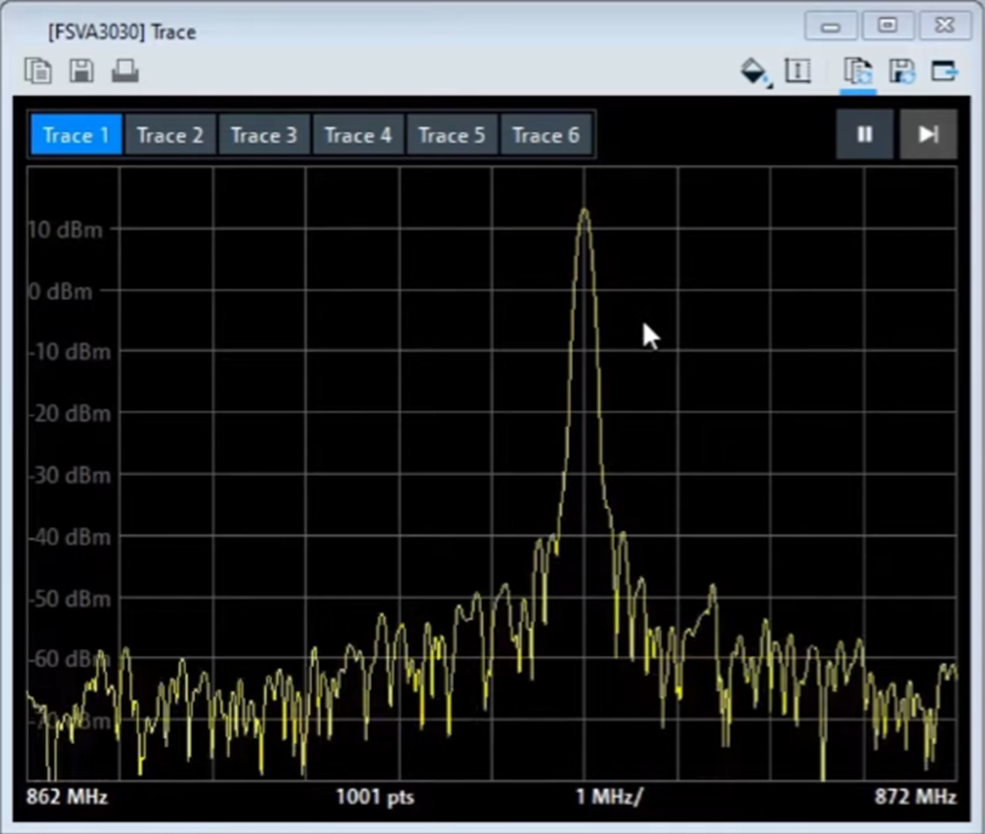
\includegraphics[width=0.7\textwidth,keepaspectratio]{out-power-meas-ex.png}
			\caption{Схема установки измерения параметров передаваемого сигнала.}
			\label{fig:out-power-meas-ex}
		\end{figure}
	\item Установить следующую частоту командой AT+TCONF=86900000:14:1:7:⅘
	\item Наблюдать спектрограмму.
	\item Повторить пункты 3-6 для других частот и амплитуд.
	\item Для измерения уровня мощности на гармониках передаваемого сигнала установим диапазон измерений от 100 МГц до 6 ГГц
		\begin{figure}[H]
			\centering
			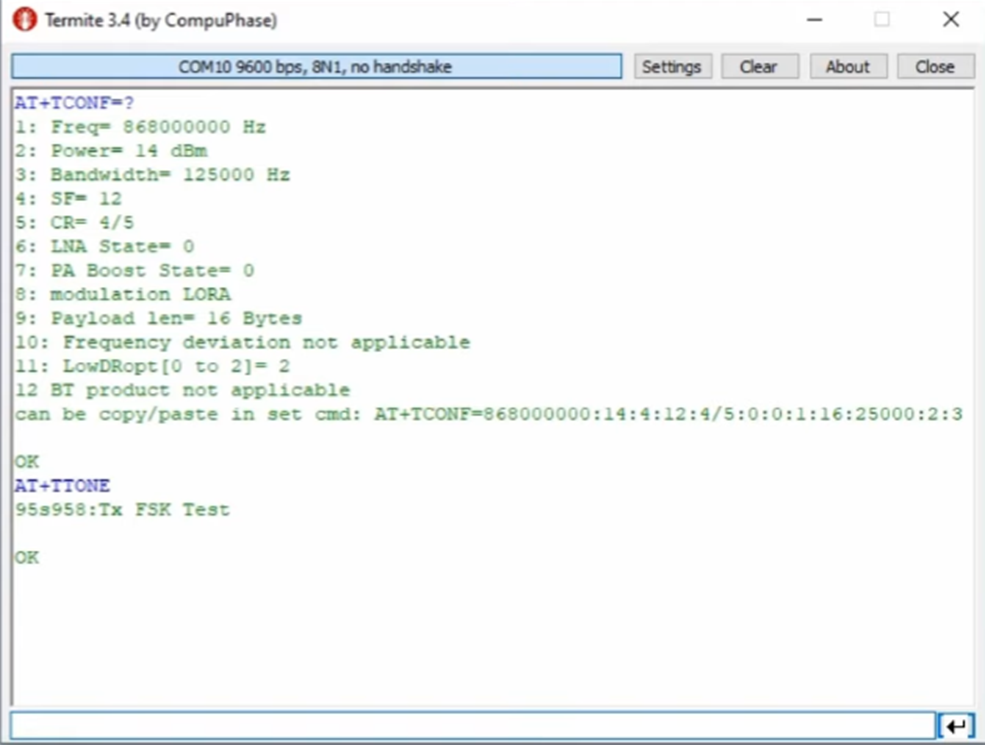
\includegraphics[width=0.6\textwidth,keepaspectratio]{out-harm-meas-ex.png}
			\caption{Схема установки измерения параметров передаваемого сигнала.}
			\label{fig:out-harm-meas-ex}
		\end{figure}	
\end{enumerate}

\subsection{Измерение параметров выходного тракта.}

\begin{figure}[H]
	\centering
	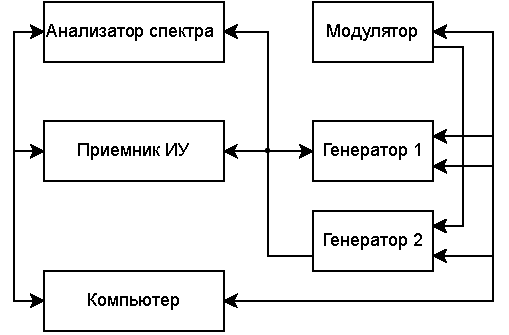
\includegraphics[width=0.6\textwidth,keepaspectratio]{RecieverMeasSch.pdf}
	\caption{Схема установки измерения чувствительности приемника.}
	\label{fig:RecieverMeasSch}
\end{figure}

\subsubsection{Подготовка к проведению измерений}

\begin{enumerate}
	\setlength\itemsep{-1ex}
	\item Включить ПК 
	\item Включить анализатор спектра и генератор. Прогреть в течение 15 минут.
	\item Откалибровать анализатор спектра
	\begin{enumerate}
		\item Открыть меню калибровки нажав кнопку CAL в разделе SYSTEM
		\item Запустить процесс калибровки, выбрав пункт SHORT CAL.
		\item Дождаться окончания процесса калибровки
	\end{enumerate}
\end{enumerate}

\subsubsection{Выполнение измерений для одного канала.}

\begin{enumerate}
	\setlength\itemsep{-1ex}
	\item Загрузить в генератор файл модулирующего сигнала и установить частоту дискретизации равной 4 ширинам полосы канала. Для 125 кГц канала требуется частота дискретизации 500 кГц. Для полосы 250 кГц, соответственно, 1 МГц.
	\item Включить генерацию центральной частоты и модуляцию.
	\item Включить исследуемое устройство и подключить его к ПК.
	\item Запустить терминал. 
	\item Отправить на ИУ AT-команды
	\begin{enumerate}
		\setlength\itemsep{-1ex}
		\item AT+TCONF=868900000:14:1:7:4/5 (установить частоту 868,9 МГц, мощность 14 дБм, полосу 125кГц, SF=7, CR=4/5)
		\item AT+TRX=50 (ожидать приём 50 пакетов)
	\end{enumerate}
	\item Дождаться возвращения в терминал вычисленного процента пакетной ошибки. 
	\item Если процент ошибок менее 1\% – уменьшить мощность генерируемого сигнала на 1 дБ.
	\item Повторять пункты 5 и 6 до тех пор, пока количество ошибок не превысит 1\%. Уровень мощности генерируемого сигнала будем считать первым значением чувствительности. 
	\item Продолжать исследование до тех пор, пока количество ошибок не превысит 15\%. Уровень мощности генерируемого сигнала будем считать вторым значением чувствительности. 
	
\end{enumerate}

\subsubsection{Выполнение измерений для двух каналов.}

\begin{enumerate}
	\item Загрузить в генератор 1 файл модулирующего сигнала (SF=7, CR=4/5, W=125 кГц) и установить частоту дискретизации равной 500 кГц. 
	\item Загрузить в генератор 1 файл модулирующего сигнала (SF=7, CR=4/5, W=250 кГц) и установить частоту дискретизации равной 1000 кГц. 
	\item Включить генерацию центральной частоты и модуляцию на обоих генераторах.
	\item Включить исследуемое устройство и подключить его к ПК.
	\item Запустить терминал. 
	\item Отправить на ИУ AT-команды
	\begin{enumerate}
		\item AT+TCONF=868900000:14:1:7:4/5:1 (установить частоту 868,9  МГц, мощность 14 дБм, полосу 125 кГц, SF=7, CR=4/5, фильтр 1)
		\item AT+TCONF=868900000:14:2:7:4/5:2 (установить частоту 868,9 МГц, мощность 14 дБм, полосу 250 кГц, SF=7, CR=4/5, фильтр 2)
		\item AT+TRX=50 (ожидать приём 50 пакетов)
	\end{enumerate}
	\item Дождаться возвращения в терминал вычисленного процента пакетной ошибки. 
	\item Если процент ошибок менее 1\% – уменьшить мощность генерируемого сигнала на 1 дБ.
	\item Повторять пункты 5 и 6 до тех пор, пока количество пакетных ошибок одного из каналов не превысит 1\%. Уровень мощности генерируемого сигнала будем считать первым значением чувствительности по данному каналу.
	\item Продолжать уменьшать мощность второго канала до тех пока, пока количество ошибок  не превысит 1\%.
	\item Продолжать исследование обоих каналов для 15\% уровня пакетных ошибок. Уровень мощности генерируемого сигнала будем считать вторым значением чувствительности. 
\end{enumerate}















